\documentclass[parskip=full]{scrartcl}
\usepackage[T1]{fontenc}    % avoid garbled Unicode text in pdf
\usepackage[utf8]{inputenc} % use utf8 file encoding for TeX sources
\usepackage[german]{babel}  % german hyphenation, quotes, etc
\usepackage{hyperref}       % detailed hyperlink/pdf configuration
\hypersetup{                % ‘texdoc hyperref‘ for options
pdftitle={PSE: Entwicklung eines relationalen Debuggers - Implementierungsdokument},%
,%
}
\usepackage{graphicx}       % provides commands for including figures
\usepackage{csquotes}       % provides \enquote{} macro for "quotes"
\usepackage[nonumberlist]{glossaries}     % provides glossary commands
\usepackage{enumitem}
\usepackage{xcolor}
\usepackage{lscape}
\newcommand\frage[1]{\textcolor{red}{#1}}


\font\myfont=cmr12 at 16pt

\title{
	\vspace{2cm}
	\myfont 
	Praxis der Softwareentwicklung:\\ 
	Entwicklung eines relationalen Debuggers\\
}
\subtitle{
	\vspace{1cm}
	\myfont
	Implementierungsdokument
}
\author{
	\vspace{1cm} \\
	Benedikt Wagner\\
	\texttt{udpto@student.kit.edu}
	\and \vspace{1cm} \\ Chiara Staudenmaier\\
	\texttt{uzhtd@student.kit.edu}
	\and Etienne Brunner\\
	\texttt{urmlp@student.kit.edu}
	\and Joana Plewnia\\
	\texttt{uhfpm@student.kit.edu} 
	\and Pascal Zwick\\
	\texttt{uyqpk@student.kit.edu}
	\and Ulla Scheler\\
	\texttt{ujuhe@student.kit.edu}
	\vspace{1cm}
	\and Betreuer: Mihai Herda, Michael Kirsten
	\vspace{4cm}
}


\begin{document}
\clearpage
\maketitle
\pagenumbering{gobble}
\newpage

\tableofcontents
\newpage
\pagenumbering{arabic}

\section{Einleitung}
Dieses Dokument beschreibt die Ergebnisse der Implementierungsphase (\textit{08.01.-02.02.2018}) im Rahmen des Moduls Praxis der Softwareentwicklung (PSE) am Lehrstuhl \enquote{Anwendungsorientierte formale Verifikation - Prof. Dr. Beckert} am Karlsruher Institut für Technologie (KIT).\\
Hierbei handlet es sich um die Implementierung des Produkts \textit{DIbugger}, welches im Pflichtenheft definiert und während der Entwurfsphase entworfen wurde.

\begin{figure}[!h]
\centering

\includegraphics[width=0.8\textwidth]{../Plichtenheft/logo_nongi.png}
\caption{Produktlogo}
\end{figure}

\section{Zeitablauf}
Um eine reibungslose Implementierung zu ermöglichen, muss ein gut durchdachter Zeitablauf existieren.
Dieser wurde folgendermaße umgesetzt:\\
Begonnen wurde mit dem \textit{FileHandler} und dem \textit{UserInterface}. Diese konnten unabhängig voneinander implementiert werden.
Aus Zeitgründen verschob sich der Start der \textit{Control} Implementierung um wenige Tage.
Die Unterpakete der \textit{DebugLogic} wurden in planmäßiger Reihenfolge begonnen. Dabei sei zu beachten, dass die \textit{DebugControl} nun parallel zum \textit{Interpreter} entwickelt worden ist.
%Aufgrund des Vergessens von simplen Getter / Setter Methoden während des Entwurfs des Pakets \textit{FileHandler.Facade} hat sich die angedachte Entwicklungszeit stark vergrößert, da immer wieder kleine Änderungen vorgenommen werden mussten.%
Der aufwändigste Teil der Implementierung war, wie auch im Entwurf erarbeitet, der \textit{Interpreter}. Insgesamt gestaltete sich aber auch die Benutzeroberfläche des Paketes \textit{UserInterface} als etwas aufwändiger.
Das nun folgende Gantt-Diagramm zeigt den Zeitverlauf in graphischer Form auf.
\begin{figure}[!h]
\centering
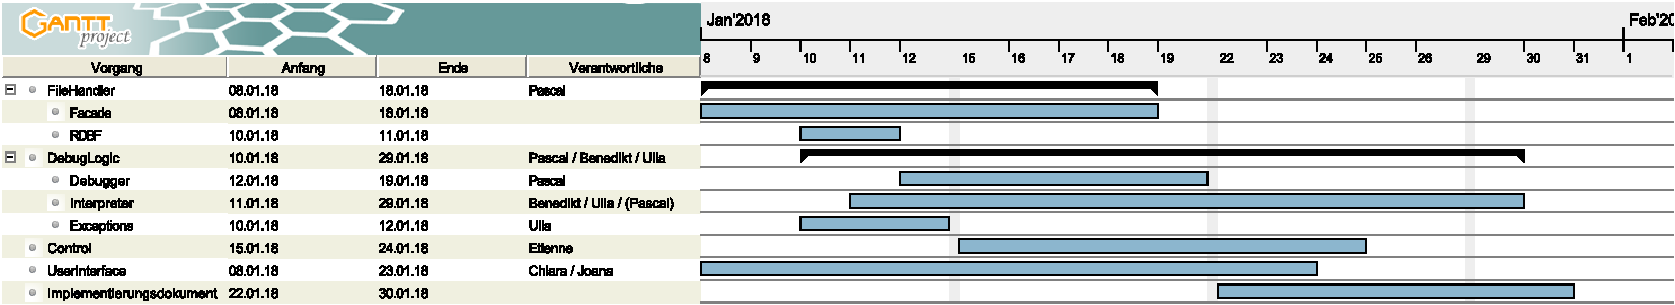
\includegraphics[width=1.0\textwidth]{ganntDiagramm_neu_crop.pdf}
\caption{Gantt-Diagramm des Zeitverlaufes}
\end{figure}

\section{Umsetzung der nichtfunktionalen-Anforderungen}

\section{Umsetzung von Entwurfsentscheidungen}
\subsection{Model-View-Control}
\subsection{Das Observerpattern}
z.B. Gui-Facade
\subsection{Singleton}
z.B. Command Panel

\subsection{Fassade}
z.B. Control-Facade

\newpage
\subsection{Strategie}
%z.B. FileWriter
\begin{figure}[!h]
\centering
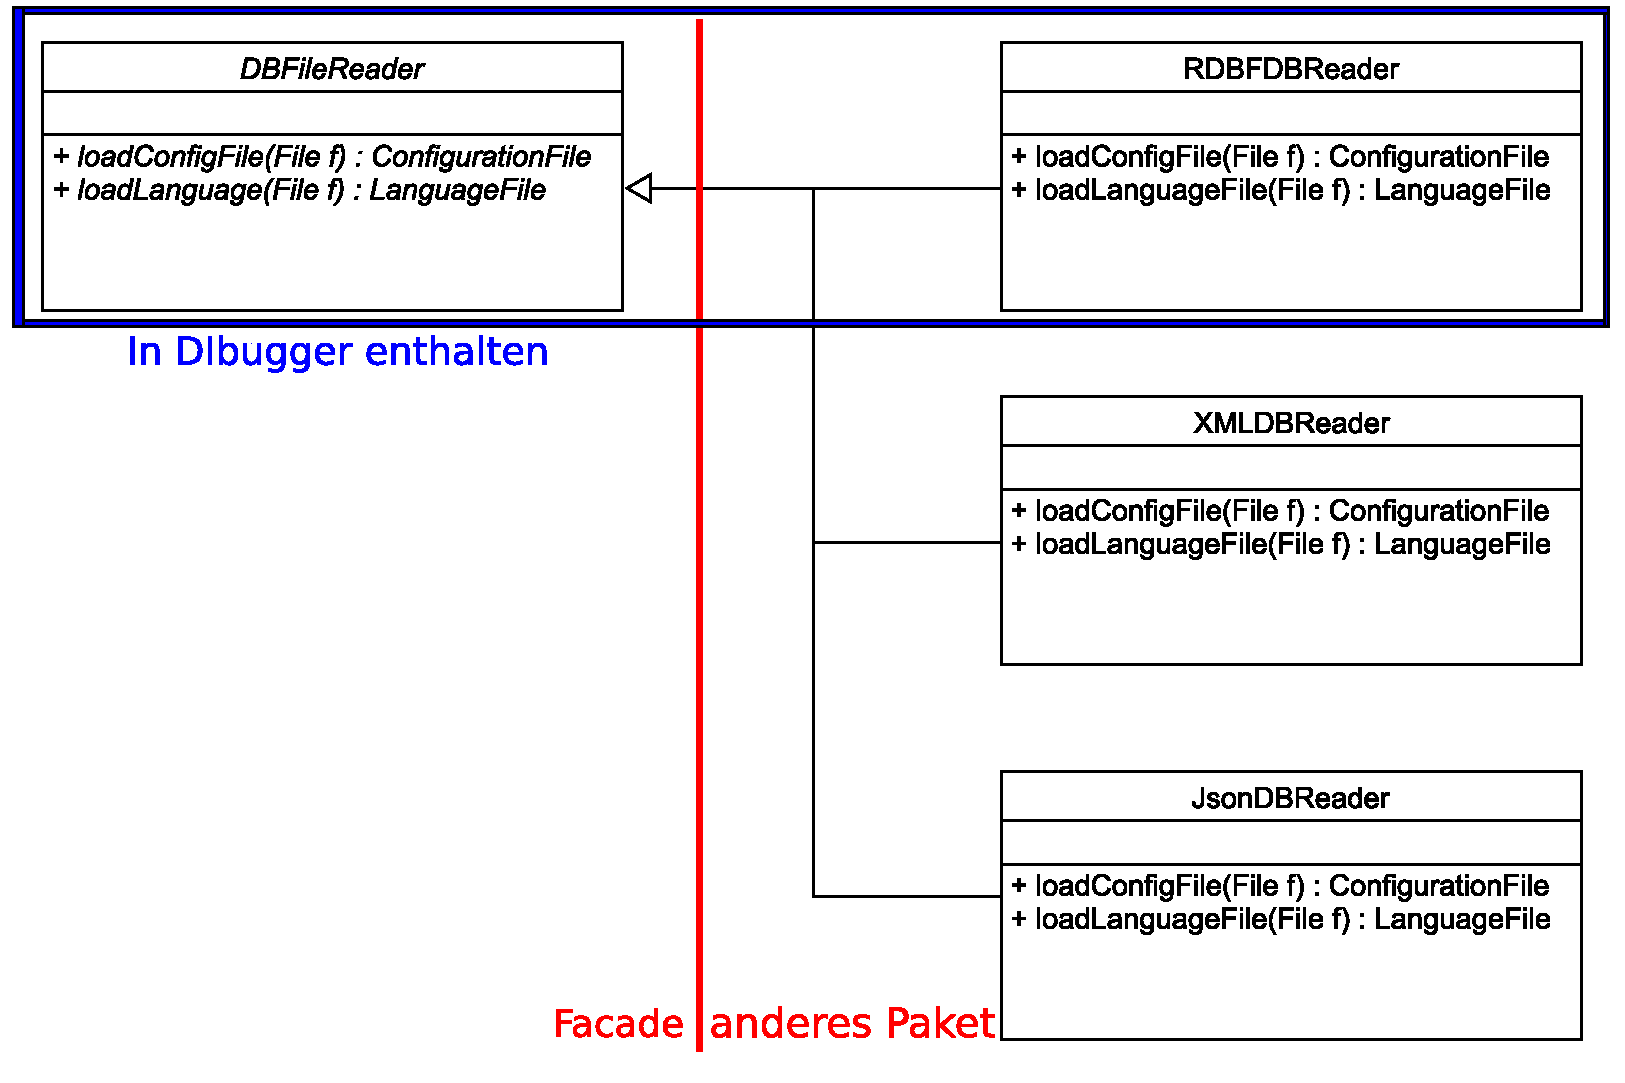
\includegraphics[width=0.8\textwidth]{document_data/Strategy_uml_d.pdf}
\begin{verbatim}
public abstract class DBFileReader {
    public abstract ConfigurationFile loadConfigFile(File f) throws FileHandlerException;
    public abstract LanguageFile loadLanguageFile(File f) throws FileHandlerException;
}
\end{verbatim}
\caption{Strategiemuster und Quelltext des DBFileReaders im Paket FileHandler}
\label{fig:strategy_fh}
\end{figure}
Wie in Abbildung \ref{fig:strategy_fh} aufgezeigt, steht der DBFileReader für den \enquote{Kopf} des Strategiemusters.
Dieser kann als abstrakte Klasse nicht erzeugt werden und stellt zwei abstrakte Methoden ohne Implementierung zur Verfügung.
Dies müssen bei der Vererbung durch eine Unterklasse, z.B. RDBFDBFileReader, XMLDBFileReader, JsonDBFileReader usw., überschrieben und vollständig Implementiert werden.
Dadurch können unter Vorraussetzung einer korrekten Implementierung der beiden Methoden weitere Dateiformate hinzugefügt werden.
Dies gilt ebenso für die Klassen \textit{DBFileWriter, PropertiesFileReader und PropertiesFileWriter}. Sie sind ähnlich aufgebaut zu der hier gezeigten Klasse.
\subsection{Die Visitor im Interpreter} Der Entwurf sah im Paket \textit{Interpreter} zwei Klassen vor, die das Visitor Pattern umsetzen. Die beiden Klassen \textit{CommandGenerationVisitor} und \textit{TermGenerationVisitor} sind Unterklassen der von Antlr generierten Klasse \textit{WlangBaseVisitor<T>}, wobei der Generic hier angibt, welchen Datentyp die visit-Methoden zurückgeben. Wie es der Name andeutet ist dies zum einen die Klasse \textit{Command} und zum anderen die Klasse \textit{Term}. 
Da Terme sowohl während der Traceerzeugung (genauere Erklärung dazu ist im Entwurfsdokument Kapitel 8.10 zu finden) als auch innerhalb von Watch-Expressions und bedingten Breakpoints vorkommen, kam das Problem auf, dass der \textit{TermGenerationVisitor} zunächst sowohl vom \textit{TermsBaseVisitor} (für die im Entwurfsdokument Anhang 12.2 definierte Syntax der Watch-Expressions) als auch vom \textit{WlangBaseVisitor} (für die in Entwurfsdokument 12.1 definierte Wlang-Syntax) erben musste. In Java ist bekanntlich keine Mehrfachvererbung möglich. Zur Lösung des Problems wurden die Grammatiken zusammengefügt und entsprechend beim Verwenden eine andere Startregel angegeben. 
\subsection{Nutzung der von Antlr generierten Klassen}
In Abbildung \ref{createTerm} ist die Nutzung der von Antlr generierten Klassen im Rahmen einer Watch-Expression zu sehen. Diese ist sehr kompfortabel und weicht bei der Nutzung für die Tracegenerierung lediglich in Zeilen 70-72 ab. Hier wird dann eine andere Startregel ausgewählt und der \textit{CommandGenerationVisitor} genutzt. Im abgebildeten Code ist vorher in \texttt{this.specifier} der String, der die Watch-Expression spezifiziert. Die Klassen \textit{WlangLexer} und \textit{WlangParser} erzeugen dann einen Ableitungsbaum, den \textit{ParseTree}. Über diesen werden die oben angesprochenen Visitor geschickt.
\begin{figure}[!h]
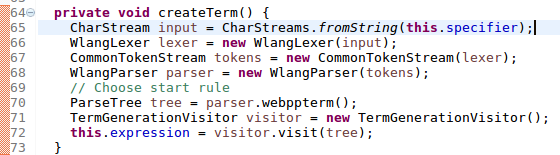
\includegraphics[width=0.7\textwidth]{document_data/createTerm.png}
\caption{Aufrufen der von Antlr erzeugten Klassen}
\label{createTerm}
\end{figure}

\subsection{Umsetzung der Commands}
Die Klassen \textit{Command} und ihre Unterklassen wurden wie im Entwurfsdokument spezifiziert als Kompositum implementiert. Dabei haben zusammengesetzte Subklassen wie der \textit{WhileCommand} immer eine \textit{addChild(Command child)}-Methode. Spannend an den Commands ist vor allem die Umsetzung ihrer \textit{run()}-Methode. Diese ist einer der wichtigsten Teile der Umsetzung des Interpreterpaketes. Sobald sich hier ein Fehler einschleicht, werden die Programmausführungen fehlerhaft. Deshalb wird es wichtig sein, in der Qualitätssicherungsphase diesen Teil besonders ausgiebig zu testen. Bereits in der Implementierung wurden die Commands durch Unittests auf ihr Verhalten überprüft. 
Als einfaches Beispiel betrachten wir in Abbildung \ref{runWhile} die run()-Methode der Klasse \textit{WhileCommand}. Hier wird der Nutzen des Kompositum Musters ersichtlich.
Zunächst wird in jedem Command der aktuelle \textit{Scope} vom hauptverantwortlichen \textit{GenerationController} \texttt{this.controller} geholt. In einfachen Befehlen (z.B. \textit{Assignment}) wird dieser einfach nur manipuliert. Hier müssen wir die Bedingung der While-Schleife auswerten, um zu sehen, ob diese sich überhaupt zu einem Boolean auswertet (Zeile 38-39). Dann prüfen wir je einmal die Bedingung und führen alle Kinder mit \textit{run()} aus. Das passiert solange die Bedingung sich zu wahr auswertet (Zeile 45-49). Da wir immer im gleichen Scope bleiben, muss die oben angesprochene Typprüfung nur einmal erfolgen.
\begin{figure}[!h]
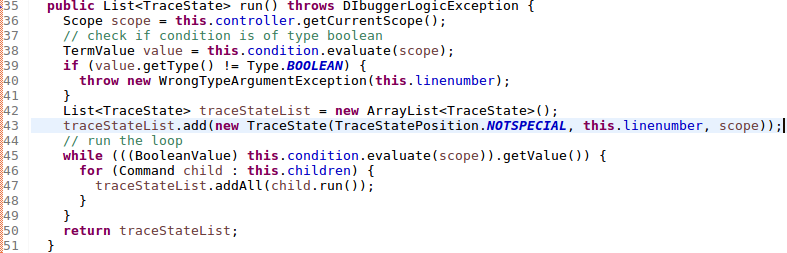
\includegraphics[width=1.0\textwidth]{document_data/runWhile.png}
\caption{run()-Methode der Klasse \textit{WhileCommand}}
\label{runWhile}
\end{figure}
\section{Änderungen zum Entwurf}

\subsection{UserInterface}
\subsection{Control}
\subsection{FileHandler}
+ FileHandlerFacade: savePropertiesFile()
\subsection{DebugLogic}
\subsubsection{Debugger}

+ DebugLogicFacade: extends Observable statt Subject
* DebugLogicFacade: notifyObservers(Object arg); suggestStepSize void statt String,

+ DebugControl: setStepSize(programID, stepSize); reset();
\subsubsection{Interpreter}
\paragraph{TraceIterator}
Ursprünglich sollte der TraceIterator mit Hilfe einer gesonderten Klasse gleichen Namens umgesetzt werden. In der Implementierung wird er nun mittels eines Java-ListIterators über die TraceState-Liste innerhalb der Klasse Trace verwirklicht. Dieser bietet dieselben Funktionalitäten, kann also in zwei Richtungen iterieren, statt nur von Anfang bis Ende Um einen Iterator über den Trace zu erhalten, wird weiterhin die Methode iterator() der Klasse Trace aufgerufen. Diese Entwurfsänderung stellt lediglich eine Vereinfachung dar, in der statt einem einzelnen\\
Änderung: Der Iterator über den Trace wurde mit Hilfe eines von Java bereitgestellen \textit{ListIterators} implementiert, den die Klasse \textit{Trace} mit ihrer \textit{iterator()}-Methode zurückgibt.
\paragraph{TermValue}abstract class statt interface \\
\paragraph{TraceState} zusätzliches Attribut: String programId, dabei auch GenerationController::generateTrace(.) hat deshalb zusätzliches Argument String programId
\section{Anhang}

\end{document}